\documentclass[10pt]{article}
\usepackage[margin=1in]{geometry}
\usepackage[T1]{fontenc}
\usepackage{lmodern}
\usepackage{microtype}
\usepackage{amsmath,amssymb}
\usepackage{booktabs}
\usepackage{graphicx}
\usepackage[numbers,sort&compress]{natbib}
\usepackage{xcolor}
\usepackage{tikz}
\usetikzlibrary{positioning,arrows.meta}
\usepackage[hidelinks]{hyperref}
\usepackage{caption}
\captionsetup{font=small,labelfont=bf}

\newcommand{\Rec}{\mathrm{R}}
\newcommand{\Acc}{\mathrm{Acc}}

\title{What a Recipient Can Recover from a Useful Prediction:\\
An Evaluation of Feature Defenses and Output Contracts on Stored Representation Models}
\author{Anonymous authors}
\date{}

\begin{document}
\maketitle

\begin{abstract}
A model that serves several purposes often releases two things to each recipient: protected features and a task prediction.
We ask, on stored Adult and HMDA models, what a recipient can recover about a declared protected attribute from the
\emph{complete} release, and how useful that release is for its task.
We evaluate purpose-specific encoders with each method's own protection check, official target LEACE, official FARE,
a capacity-matched zero-fairness FARE tree, and several output formats (full logits, logits without their common
offset, probabilities, hard decisions), using one attacker slate, held-out roles, and paired group-bootstrap intervals.
Four findings recur.
(i) Methods can pass their own checks while nonlinear recipients still recover the attribute (AUC about 0.81--0.86 under
official LEACE, against 0.82--0.87 untreated), and the purpose-specific encoders fail their own stored linear check on 12 of 42 attribute--seed
combinations.
(ii) Releasing an unchanged task output bypasses any feature defense (recovery returns to 0.76--0.79).
(iii) The frozen heads' hard decisions leak little but are also weakly useful; when every arm releases a genuinely
useful logistic-regression head fitted on its own features, the head's score under LEACE still recovers sex at 0.759
(untreated 0.774), while FARE's recovers 0.539 at an accuracy cost whose non-inferiority within one point is not established.
A same-size tree without the fairness term recovers 0.648, so on this cell the fairness term removes 0.109 AUC beyond
compression, whereas on an easier task compression reproduced most of FARE's effect.
(iv) Two recipients pooling their outputs recover more than either alone, including from decisions only.
All results are development evidence on repeatedly used data. We propose no new algorithm, no population privacy
certificate and no composition theorem.
\end{abstract}

\section{Introduction}

Representation-level defenses are usually evaluated on the representation: a linear probe, an in-training adversary,
or a certificate about classifiers that read the representation. Deployed systems release more. A recipient permitted
a purpose typically receives a task output for that purpose---a score, a probability or a decision---and often the
features that produced it. Whatever is withheld from the features may be carried by the output, and a recipient who
holds both, or who pools releases with another recipient, sees more than any one channel.

This paper reports a controlled empirical analysis of that complete view on stored models. We evaluate four bodies of
work in our repositories that were developed separately and are \emph{not} connected by any pipeline: purpose-specific
encoders with a linear protection constraint; attribute-removal and isolation work on those encoders (an erase layer,
noise, and comparisons with LEACE, INLP, LAFTR and SPLINCE); finite-release studies on later census data; and the
stored-model analyses that this paper centres on (a matched removal benchmark, an output-aware study, an output
diagnosis and the useful-head comparison). We never describe them as one evaluated architecture. The encoders use a frozen, \emph{seeded, randomly
initialised} backbone with trained per-purpose adapters and heads; the backbone is not pretrained.

\paragraph{Questions.} We organise the evidence around five questions: what each method's own protection check
establishes; what a recipient recovers from the features, the output, or both; how useful the released output is;
how much of a fair-representation method's effect is ordinary compression; and what changes when recipients combine
their releases.

\paragraph{Contributions.} (1) A common evaluation protocol (one attacker slate and endpoint discipline; roles and bootstrap differ
slightly across studies, Section~\ref{sec:protocol}) applied to the same stored models: each method's native
check, nonlinear recovery from the representation, from the complete output and from both, held-out utility of the
output actually released, a capacity-matched zero-fairness control, and recipient pairs (Section~\ref{sec:protocol}).
(2) A matched comparison in which every arm releases a deployable task head of one common family fitted on its own
features, so that recovery is read beside real utility rather than beside a probe (Section~\ref{sec:useful}).
(3) Measured findings with their adverse qualifications: an output-contract change that lowered recovery for particular
frozen heads but not in general; the compression share of FARE's effect, which differs between two cells; and
decision-level coalition gains. The individual observations---that linear protection does not stop nonlinear recovery,
that outputs leak beyond labels, that hard labels are not a defense in general, and that combined releases leak
more---are established (Section~\ref{sec:related}); our contribution is measuring them together, with utility, on the
same models.

\paragraph{Scope.} Every assessment row has been used by earlier analyses in our repositories. Registering endpoints and
committing locks before fitting does not turn these rows into fresh confirmation. Intervals are conditional on the
fitted heads and attackers. Recovery is a measured property of our attackers, not a population privacy guarantee. We
make no use of an earlier, retired bound from linear $R^2$ to classifier accuracy, and we do not claim that the public
code's default interface has been repaired: a fix exists on an unmerged branch.

\section{Setting}\label{sec:setting}

\paragraph{Stored models.} We use six stored purpose-specific encoders (Round~4 checkpoints): Adult and HMDA, encoder
seeds 0, 1 and 2. Each maps a record to a 64-dimensional representation per purpose and carries a frozen task head per
purpose. The encoders were trained with a linear (one-hot ridge $R^2\le 0.05$) constraint on declared disallowed
attributes. The primary cells are Adult \texttt{income\_prediction} with protected attribute sex and HMDA
\texttt{underwriting} with race; secondary analyses use all 14 stored purpose--attribute pairs.

\paragraph{Recipients and release contracts.} Figure~\ref{fig:recipient} shows the paths. A recipient receives (1) a
task output only; (2) features together with the output of a head fitted only on those features; or, as an adverse
control, (3) features together with the historical clean task logits of the untreated model---a bypass that a
release policy should not permit. Outputs are released in one of four formats. For a $K$-class logit vector $l$, write
the common offset $c=\frac1K\sum_k l_k$ and the centred logits $l-c\mathbf 1$; for $K=2$ the centred logits are
determined by the margin $d=l_1-l_0$. Probabilities and decisions do not depend on $c$ (softmax shift
invariance~\citep[\S4.1]{goodfellow2016deep}). The formats are \emph{full} logits, \emph{centred} logits,
\emph{probabilities}, and the \emph{hard} decision.

\begin{figure}[t]
\centering
\resizebox{\linewidth}{!}{% Recipient diagram: permitted release paths (solid) and the historical bypass (dashed red).
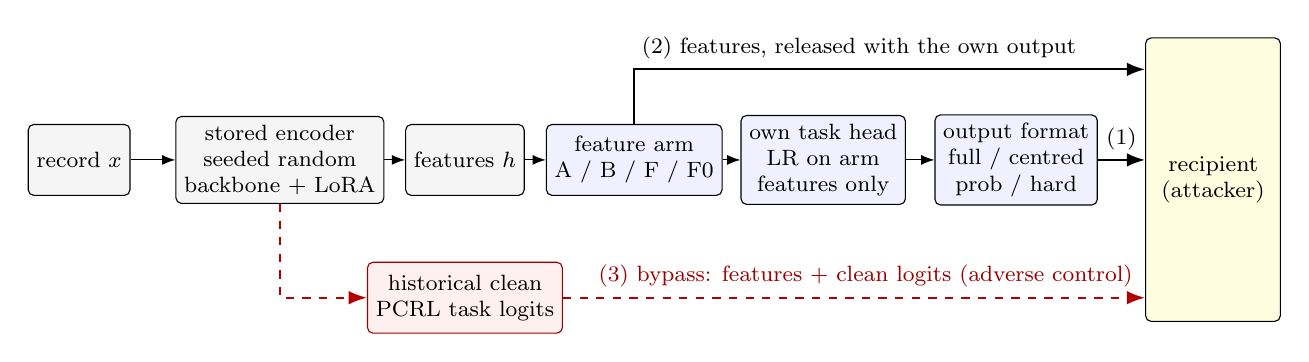
\begin{tikzpicture}[
  font=\footnotesize, >=Latex,
  box/.style={draw, rounded corners=2pt, align=center, minimum height=9mm, inner sep=3pt},
  own/.style={box, fill=black!4},
  rel/.style={box, fill=blue!6},
  bad/.style={box, fill=red!6, draw=red!60!black}]
  \node[own] (x) at (0,0) {record $x$};
  \node[own] (enc) at (2.55,0) {stored encoder\\seeded random\\backbone + LoRA};
  \node[own] (h) at (4.9,0) {features $h$};
  \node[rel] (arm) at (7.05,0) {feature arm\\A / B / F / F0};
  \node[rel] (hd) at (9.45,0) {own task head\\LR on arm\\features only};
  \node[rel] (out) at (11.9,0) {output format\\full / centred\\prob / hard};
  \node[box, fill=yellow!12, minimum height=36mm, text width=15mm] (rec) at (14.4,-0.25) {recipient\\(attacker)};
  \node[bad] (clean) at (4.9,-1.75) {historical clean\\PCRL task logits};
  \draw[->] (x) -- (enc);
  \draw[->] (enc) -- (h);
  \draw[->] (h) -- (arm);
  \draw[->] (arm) -- (hd);
  \draw[->] (hd) -- (out);
  \draw[->, thick] (out) -- node[above]{(1)} (out -| rec.west);
  \draw[->, thick] (arm.north) |- node[pos=0.72, above]{(2) features, released with the own output} (rec.west |- 0,1.15);
  \draw[->, dashed, thick, red!70!black] (enc.south) |- (clean.west);
  \draw[->, dashed, thick, red!70!black] (clean.east) -- node[pos=0.52, above, text=red!60!black]{(3) bypass: features + clean logits (adverse control)} (clean -| rec.west);
\end{tikzpicture}
}
\caption{Recipient view. Solid paths are permitted releases: (1) output only, in one of four formats; (2) features of
an arm (A untreated, B LEACE, F FARE, F0 zero-fairness FARE tree) released with the output of a task head fitted only
on those features. The dashed path (3) is the historical clean-output bypass, evaluated only as an adverse control.}
\label{fig:recipient}
\end{figure}

\paragraph{Feature arms.} A: untreated representation. B: official target LEACE~\citep{belrose2023leace}
(concept-erasure 0.2.4), fitted on the owner's \texttt{defense\_fit} role. F: official FARE~\citep{jovanovic2023fare},
whose nominee is chosen from a frozen grid on validation only among configurations within one point of untreated
validation accuracy; its release is the one-hot tree cell. F0: the same FARE configuration with fairness weight zero,
i.e.\ a tree of the same budget that only compresses. Gaussian noise at a validation-selected scale appears in the
benchmark. No defense grid was expanded and no candidate was re-selected after assessment.

\section{Related work}\label{sec:related}

\paragraph{Concept erasure and its evaluation.} Linear concept erasure aims to stop linear classifiers from recovering a
concept: INLP~\citep{ravfogel2020inlp} by iterative nullspace projection, R-LACE~\citep{ravfogel2022rlace} through a
linear minimax game, and LEACE~\citep{belrose2023leace}, which guarantees it in closed form with minimal change to the
representation. Such guarantees do not extend to nonlinear
recipients: INLP and R-LACE report nonlinear recovery after linear erasure, kernelized erasure does not transfer
across kernels~\citep{ravfogel2022kernel}, and LEACE restricts its claim to linear adversaries. Adversarially trained
representations show the same pattern: post-hoc attackers recover what the in-training adversary could
not~\citep{elazar2018adversarial,song2020overlearning}, and independent post-hoc adversaries are a standard
check~\citep{moyer2018invariant}. Our LEACE measurements are a further instance, not a refutation of LEACE's theorem.

\paragraph{Leakage through task outputs.} Model-inversion and attribute-inference attacks exploit confidence
scores~\citep{fredrikson2014pharmacogenetics,fredrikson2015model}; label-only attacks can match confidence-based
ones~\citep{mehnaz2022sensitive}, and masking confidences does not stop label-only membership
inference~\citep{choquettechoo2021label}. \citet{wang2019balanced} compare leakage from predictions with that implied
by the true labels at matched task performance; we report a label-only reference in the same spirit. A multiclass
log-linear head on a linearly guarded representation can still reveal the erased concept, although a binary one
cannot~\citep{ravfogel2023loglinear}.
Many black-box attribute-inference results do not exceed imputation~\citep{jayaraman2022imputation}, so we report
constant and label-only references. Coarsening outputs, e.g.\ rounding confidences~\citep{fredrikson2015model}, is an
old countermeasure; releasing probabilities rather than logits leaves calibration~\citep{guo2017calibration} and every
proper task loss unchanged.

\paragraph{Fair representations and trade-offs.} When the label depends on the protected attribute, fair
representations trade accuracy for protection~\citep{zhao2019inherent,zhao2022inherent}, and a release useful for a
task reveals what the task's label reveals~\citep{stadler2024lpl}. Adversarial methods such as
LAFTR~\citep{madras2018laftr} lack guarantees against unseen classifiers; FCRL~\citep{gupta2021fcrl} evaluates with a
common downstream protocol. FARE~\citep{jovanovic2023fare} restricts the encoder to a finite partition and certifies the
demographic-parity distance of any classifier that reads only the cell; its authors note that restricted encoders lose
information and compare fairness-unaware $k$-means encoders. We add a same-budget zero-fairness tree and measure
attribute recovery from the complete release.

\paragraph{Combining releases.} Combining independent releases is a classical route to
breaches~\citep{ganta2008composition}; combining a biased and a debiased version of one model raises attribute
inference~\citep{tian2025fairnessprivacy}; collusion-aware mechanisms exist for sequential finite-alphabet
releases~\citep{taylor2026collusion}. We measure the purpose-permission version, as a property of our attackers.

\paragraph{Position.} In a bounded reading of the closest work, we did not find one protocol that applies, on the same
stored models, each method's native check, nonlinear recovery from representation and complete output, the released
output's held-out utility, a capacity-matched zero-fairness control, and recipient pairs. FARE is closest on matched
utility and compression, \citet{wang2019balanced} on utility-qualified output leakage, and
\citet{tian2025fairnessprivacy} on combined releases. This is a gap in a bounded search, not evidence of priority.

\section{Evaluation protocol}\label{sec:protocol}

\paragraph{Roles.} The output-aware, output-diagnosis and useful-head analyses use the same record-group roles: \texttt{defense\_fit} (owner side: LEACE maps, FARE
trees, task heads, with a 20\% head holdout for head selection), \texttt{attacker\_fit} and \texttt{attacker\_val}
(attacker fitting and selection), and \texttt{assessment} (scoring only: 5{,}243 Adult and 4{,}764 HMDA records).
Records that also occur in the encoder's training split are excluded from every scored role (17 Adult and 42 HMDA test
records), and a further 20\% of \texttt{attacker\_fit} groups is reserved for FARE certification. No sensitive
assessment label selects a release, grouping, penalty, attacker or utility probe. The earlier matched benchmark used
the uncleaned roles (assessment 5{,}250 Adult and 4{,}778 HMDA records; the overlapping records retained and
disclosed; its decisions were stable when they were removed).

\paragraph{Attackers and recovery.} Every surface is attacked by the same slate: logistic regression (5 regularisation
values), gradient-boosted trees (20 configurations) and an MLP (18). The nonlinear attacker is the better of the tree
and MLP families on \texttt{attacker\_val} log loss, refitted at three attacker seeds. Recovery is the macro one-vs-rest
AUC on assessment over supported classes, averaged over attacker seeds and then encoder seeds. For features plus output,
candidates that ignore one part are also eligible on validation. For finite releases we additionally fit a
cell-conditional attacker and report it descriptively. Banks over output formats select on validation only.

\paragraph{Utility.} We report the accuracy, balanced accuracy, minority recall, log loss and gain over the constant
(majority class on \texttt{attacker\_fit}) of the \emph{deployed} head whose output is released, and, separately, the
accuracy of a common refitted probe used by earlier analyses.

\paragraph{Native checks.} The encoders' stored check is in-sample one-hot ridge $R^2\le0.05$; LEACE's implementation
bound is a whitened residual cross-covariance below its tolerance on \texttt{defense\_fit}; FARE's is its
demographic-parity certificate on the certification role.

\paragraph{Inference.} Each endpoint is a mean over encoder seeds of a per-seed statistic. In the output-diagnosis and
useful-head studies, standard errors come from 1{,}999 paired multinomial bootstrap replicates over assessment record
groups, shared by every unit, and intervals are simultaneous two-sided 95\% Bonferroni normal intervals over the
endpoint family; the matched benchmark and the output-aware study used one-sided Bonferroni percentile bounds from
20{,}000 group-bootstrap replicates (the bounds in Table~\ref{tab:summary} from those studies are of that kind). In all studies and an endpoint passes only if its lower bound exceeds
its registered target. Utility targets are a non-inferiority margin of $-0.01$, a gain of $0.03$, and the retention
contrast $\Acc(\text{arm})-0.8\,\Acc(A)-0.2\,\Acc(\text{const})>0$; recovery targets are $0.02$ AUC (the earlier frozen-head usefulness endpoints used a gain target of 0.01). An interval that
excludes zero but not the target is reported as a smaller difference below the target, never as ``no difference''.
Each study's protocol, code, inputs, unit list and endpoint families were committed and pushed before its first fit;
an independent replay that does not import the runner's code recomputed every primary result.

\section{Results}\label{sec:results}

Table~\ref{tab:summary} summarises the earlier stored-model analyses; Sections~\ref{sec:useful}--\ref{sec:pairs}
report the new useful-head comparison and the combined findings.

\begin{table}[t]
\centering\small
\caption{Key contrasts from the stored-model analyses (means over three encoder seeds; simultaneous lower bounds in
parentheses where an endpoint was registered).}\label{tab:summary}
\begin{tabular}{@{}p{7.0cm}cc@{}}
\toprule
Quantity & Adult income / sex & HMDA underwriting / race\\
\midrule
Encoders' own linear check fails (pair$\times$seed, all 14 pairs) & \multicolumn{2}{c}{12 of 42}\\
Nonlinear recovery, untreated features & 0.815 & 0.870\\
Nonlinear recovery, LEACE features (benchmark roles) & 0.817 & 0.863\\
Noise at $\sigma^*$, features only / plus clean outputs & 0.528 / 0.778 & 0.513 / 0.758\\
Full logits vs hard decision (frozen head) & 0.776 vs 0.513: +0.263 (0.249) & 0.768 vs 0.505: +0.262 (0.254)\\
Offset removed: full-bank minus offset-free bank & +0.072 (0.062) & +0.067 (0.060)\\
\quad per encoder seed & 0.079 / 0.064 / 0.072 & 0.058 / $-$0.000 / 0.143\\
Frozen head: accuracy gain over constant (target 0.01) & 0.039 (0.031) & 0.016 (0.0098), not established\\
FARE vs LEACE features (output-aware roles) & 0.550 vs 0.812 & 0.501 vs 0.864\\
Zero-fairness tree (same budget), features & 0.645 & 0.607\\
FARE features plus historical clean outputs & 0.788 & 0.768\\
\bottomrule
\end{tabular}
\end{table}

\paragraph{Native checks and recovery outside their scope.} Three outcomes must be kept apart: a method failing its own
test, its test holding while recovery occurs outside its scope, and an output bypass. The encoders fail their own
stored linear check on 12 of 42 untreated attribute--seed combinations, including HMDA underwriting/race on two of
three seeds. Official LEACE meets its bound on all 60 maps and its held-out squared top canonical correlation
$\rho_1^2$ is near zero (Adult 0.0006, HMDA 0.0001, on one already-used held-out split), yet nonlinear recovery changes
by less than 0.01 AUC (Adult $+0.002$, HMDA $-0.007$; the HMDA interval excludes zero; Table~\ref{tab:summary}). FARE's native
certificate was unavailable, vacuous or weak (Adult bounds about 0.50) at the available certification sizes; its only
informative bound (0.175) belongs to a degenerate single-cell HMDA nominee.

\paragraph{Outputs and the bypass.} Outputs leak beyond the true label: output-only recovery exceeds the label-only
reference by 0.177 (Adult) and 0.236 (HMDA). Whatever is done to the features, releasing the historical clean output
restores recovery to 0.76--0.79 (noise, FARE). Changing the features cannot remove what an unchanged output carries.

\paragraph{Usefulness qualifies low decision-level recovery.} Hard decisions of the frozen heads leak little (0.513 /
0.505), but those decisions are weakly useful: the Adult frozen head gains 3--5 accuracy points over a constant and
recalls 14--22\% of high earners; HMDA underwriting usefulness is not established; and the HMDA fair\_lending head
predicts the same class for everyone, although its scores still vary and are informative about race and sex (centred-logit recovery
0.646 and 0.655). Low decision-level recovery here coincides with decisions that barely beat a constant.

\paragraph{An output-contract measurement, not a general method.} Withholding the common logit offset---which changes no
probability, decision or task loss---lowered recovery by 0.072 (Adult) and 0.067 (HMDA) AUC. The effect appeared on 5
of 6 primary encoder seeds (not on the collapsed HMDA seed~1) and on 5 of 14 stored pairs; it was not established for any of the six multiclass
Adult pairs, although it passed for the five-class HMDA pricing head with race. For a refitted logistic-regression head whose logits are log-probabilities, the offset is a function of the
margin, so the effect is zero by construction; that head is about twice as useful (gain 0.083) and its margin alone
recovers 0.773.

\subsection{Matched useful-head comparison}\label{sec:useful}

\paragraph{Design.} On Adult income/sex, every arm releases the output of a logistic-regression head from one common
family (regularisation grid fitted on \texttt{defense\_fit} minus a holdout, selected on holdout log loss) whose only
runtime input is that arm's features. The heads, LEACE maps and FARE trees are reused unchanged. Full-logit output-only,
features-only, features-plus-full-output and bypass surfaces are reused, hash-verified, from the output-aware study,
whose exploratory tables had already reported their levels. The centred, probability and hard surfaces and the banks
are new: 84 attacker units (3{,}924 model fits), run after the protocol lock. Because the heads emit log-probabilities, their full logits,
centred margin and probabilities carry identical information (verified to $10^{-12}$); the 19 primary endpoints use
the centred and hard formats.

\begin{figure}[t]
\centering
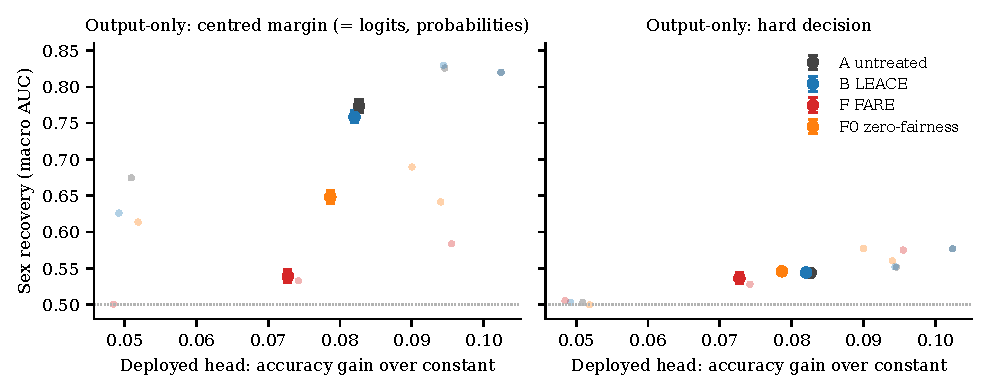
\includegraphics[width=\linewidth]{figures/fig_useful_head.pdf}
\caption{Useful-head comparison on Adult income/sex. Each arm releases the output of a deployable logistic-regression
head fitted on its own features. Large markers: means over three encoder seeds with 90\% intervals; small markers:
individual seeds. The dotted line is chance.}\label{fig:useful}
\end{figure}

\begin{table}[t]
\centering\small
\caption{Primary useful-head endpoints (19; Bonferroni $z=3.008$). Recovery is output-only. n.e.: not established;
``excl.\ 0'': the interval excludes zero but not the target.}\label{tab:useful}
\begin{tabular}{@{}lccl@{}}
\toprule
Endpoint (target) & Point & Interval & Decision\\
\midrule
$\Acc(B)-\Acc(A)$ ($>-0.01$) & $-0.0006$ & [$-0.0016$, 0.0003] & pass\\
$\Acc(F)-\Acc(A)$ ($>-0.01$) & $-0.0099$ & [$-0.0152$, $-0.0046$] & n.e.\\
$\Acc(F_0)-\Acc(A)$ ($>-0.01$) & $-0.0040$ & [$-0.0086$, 0.0005] & pass\\
Gain over constant, B / F / F0 ($>0.03$) & 0.082 / 0.073 / 0.079 & $\ge$0.067 / 0.057 / 0.063 & pass\\
Retention, B / F / F0 ($>0$) & 0.016 / 0.007 / 0.013 & $\ge$0.013 / 0.001 / 0.007 & pass\\
\midrule
Centred: $\Rec(A)-\Rec(B)$ ($>0.02$) & 0.015 & [0.011, 0.019] & n.e.\ (excl.\ 0)\\
Centred: $\Rec(A)-\Rec(F)$ & 0.234 & [0.217, 0.252] & pass\\
Centred: $\Rec(A)-\Rec(F_0)$ & 0.125 & [0.112, 0.139] & pass\\
Centred: $\Rec(B)-\Rec(F)$ & 0.220 & [0.201, 0.238] & pass\\
Centred: $\Rec(F_0)-\Rec(F)$ & 0.109 & [0.092, 0.126] & pass\\
Hard: all five contrasts & $-0.002$ to 0.010 & lower bounds $<0$ & n.e.\\
\bottomrule
\end{tabular}
\end{table}

\paragraph{Utility.} All four heads are genuinely useful (Figure~\ref{fig:useful}, Table~\ref{tab:useful}): accuracy
0.832 (A), 0.831 (B), 0.822 (F) and 0.828 (F0) against a constant of 0.749, with balanced accuracy 0.72--0.73 and about
half of high earners recalled. LEACE and the zero-fairness tree are non-inferior within one point; FARE is not
established as non-inferior (lower bound $-0.015$), because seed~2 loses 2.0 points. FARE passes the gain and
retention criteria, the latter narrowly.

\paragraph{Recovery from useful scores.} The untreated head's score recovers sex at 0.774 and the LEACE head's at
0.759: a smaller difference of 0.015, below the registered target, carried by seed~0 alone. FARE's head recovers 0.539
and the zero-fairness tree's 0.648. Of FARE's 0.234 reduction, compression accounts for 0.125 and the fairness term for
a further 0.109, on every seed. Post hoc and descriptively, a linear attacker on the untreated head's margin recovers
only 0.515, while nonlinear attackers on the same scalar recover 0.773. This is consistent with, but does not establish,
the reading that the sex signal left in the score is not linearly decodable and so lies outside a linear eraser's scope.

\paragraph{Recovery from useful decisions.} When only the decision is released, every arm recovers 0.536--0.546 and no
contrast is established. The decision has the same accuracy as the score it comes from. Post hoc and descriptively, the
untreated head's decisions leak about as much as FARE's scores (difference $+0.005$, 90\% interval [$-0.003$, 0.013])
while being about one point more accurate.

\paragraph{Complete release.} With features plus own output, the features dominate (A 0.816, B 0.817, F 0.550, F0
0.646); withholding the offset changes nothing for these heads; and adding the historical clean logits to F or F0
features restores recovery to 0.788 / 0.789.

\paragraph{Pre-registered predictions.} Four of the ten primary recovery predictions were correct. The predictions
were registered after full-logit recovery of these same heads had been reported as exploratory in the output-aware
study, and that was not disclosed in the protocol; we disclose it here. We predicted a
larger LEACE effect on the score, a smaller fairness-term effect, and established hard-decision contrasts; all three
were wrong.

\subsection{How much of FARE's effect is compression?}\label{sec:compression}

The answer differs by cell. On Adult income/sex features (output-aware analysis), the zero-fairness tree recovers 0.645
against FARE's 0.550 and LEACE's 0.812. On the head outputs above, the fairness term removes 0.109 beyond compression.
On an easier task chosen by a validation-only screen (Adult employment group with age group protected; accuracy 0.974
for FARE vs 0.975 untreated against a constant of 0.277), FARE's complete-release recovery is 0.151 below LEACE's, but
the zero-fairness tree reproduces most of that reduction: FARE had a smaller additional improvement of 0.0074
[0.0019, 0.0129], below the registered 0.02 target. That task is easy, but no single input column determines it. A
claim about a fairness term therefore needs its capacity-matched twin.

\subsection{Combining recipients}\label{sec:pairs}

\begin{figure}[t]
\centering
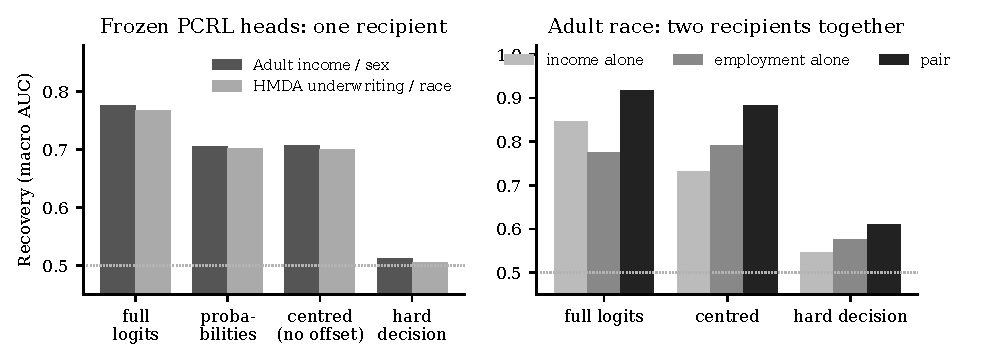
\includegraphics[width=\linewidth]{figures/fig_formats_pairs.pdf}
\caption{Left: recovery from the frozen heads' outputs by release format (Adult income/sex, HMDA underwriting/race).
Right: race recovery on Adult from the income recipient, the employment recipient and both pooled, by format.}
\label{fig:pairs}
\end{figure}

Two Adult recipients, each permitted only its own task output (income; employment group), pool their outputs to
recover race, which is disallowed for both (Figure~\ref{fig:pairs}). The pair beats both single recipients by more
than 0.02 AUC under every format: full logits 0.917 vs 0.845, centred 0.883 vs 0.792, and hard decisions 0.611 vs
0.576 (pair minus best single $+0.034$, lower bound 0.023, the weakest of six passes). We report absolute pair recovery
and its increment over the strongest single release separately. On seed~2 under full logits, validation selected the
income-only attacker for the pair, so that seed's pair-minus-income difference is exactly zero.

\section{Discussion}\label{sec:discussion}

\paragraph{What helped while preserving utility.} LEACE preserved the deployed head's accuracy (difference $-0.0006$, lower bound $-0.0016$;
non-inferior within one point) and passed its
own bound, but it barely changed what that head's score reveals (0.759 vs 0.774). The zero-fairness tree preserved
accuracy within one point and reduced score-level recovery to 0.648; FARE reduced it further to 0.539, with an
accuracy cost not shown to be within one point. Releasing only the decision preserved accuracy by construction and gave
the lowest recovery for every arm, but discards scores that a recipient may need.

\paragraph{What was compression or weak usefulness.} Part of FARE's effect is compression, by an amount that depends on
the cell. The earlier ``decisions leak little'' pattern was observed on decisions that barely beat a
constant; with useful heads, decisions still recovered only 0.536--0.546, so weak usefulness is not the whole story.

\paragraph{A measured gap (post hoc, descriptive).} At matched accuracy (within one point, established), the lowest score-level recovery among
the evaluated arms is the zero-fairness tree's 0.648, while the untreated decision---same accuracy, no scores---recovers
0.544. A method that released calibrated, useful scores with recovery near the decision's level would close a measured
gap of about 0.10 AUC on this cell. We do not claim such a method exists, nor that it is impossible.

\paragraph{Strongest favourable and adverse comparisons.} Favourable: on the useful-head cell the fairness term removes
0.109 AUC beyond a capacity-matched tree on every seed, and, post hoc, FARE's score leaks about as little as the
untreated decision. Adverse: FARE's accuracy is not shown to be within one point; any defense is bypassed by an unchanged output;
two recipients recover more than one, even from decisions.

\section{Limitations, reproducibility, ethics and LLM assistance}\label{sec:limits}

\paragraph{Limitations.} Two datasets, a small number of primary cells and three encoder seeds; the encoder seeds differ
strongly (one HMDA encoder is heavily collapsed). All assessment rows were used before; nothing here is fresh
confirmation. Intervals are conditional on fitted heads and attackers and omit retraining variance. FARE is applied to
stored representations rather than raw inputs. Rare HMDA race groups are not estimable. We test no repeated-query or
adaptive-query attacker. Several observations in Section~\ref{sec:useful} are post hoc and labelled as such.

\paragraph{Reproducibility.} For every study the protocol, code pin, admitted-input hashes, unit list, endpoint
families and budget were committed before fitting; each study's result tables, inference code, verification replay and
hash indexes are in the anonymous repository. Per-record outputs, weights and checkpoints are kept privately with
hash indexes and a verified offline copy. The useful-head comparison used about 0.2 CPU-hours on a laptop.

\paragraph{Ethics.} We study recovery of declared protected attributes from public benchmark data to inform release
policies. Attack code is standard; we release no per-person predictions.

\paragraph{LLM assistance.} A large language model assisted with code, analysis scripts, independent-replay scripts,
literature checking and drafting. All numbers were produced by committed code and checked by a replay that does not
import the analysis code; the authors are responsible for the content.

\bibliographystyle{plainnat}
\bibliography{references}

\end{document}
